%%%%%%%%%%%%%%%%%%%% author.tex %%%%%%%%%%%%%%%%%%%%%%%%%%%%%%%%%%%
%
% sample root file for your "contribution" to a contributed volume
%
% Use this file as a template for your own input.
%
%%%%%%%%%%%%%%%% Springer %%%%%%%%%%%%%%%%%%%%%%%%%%%%%%%%%%%%%%%%%


%% RECOMMENDED %%%%%%%%%%%%%%%%%%%%%%%%%%%%%%%%%%%%%%%%%%%%%%%%%%%
\documentclass[graybox]{svmult}
%
%% choose options for [] as required from the list
%% in the Reference Guide
%
\usepackage{mathptmx}       % selects Times Roman as basic font
\usepackage{helvet}         % selects Helvetica as sans-serif font
\usepackage{courier}        % selects Courier as typewriter font
\usepackage{type1cm}        % activate if the above 3 fonts are
                             % not available on your system
%
\usepackage{makeidx}         % allows index generation
\usepackage{graphicx}        % standard LaTeX graphics tool
%                             % when including figure files
\usepackage{multicol}        % used for the two-column index
\usepackage[bottom]{footmisc}% places footnotes at page bottom
%
%% see the list of further useful packages
%% in the Reference Guide
%
\makeindex             % used for the subject index
%                       % please use the style svind.ist with
%                       % your makeindex program
%
%%%%%%%%%%%%%%%%%%%%%%%%%%%%%%%%%%%%%%%%%%%%%%%%%%%%%%%%%%%%%%%%%%%%%%%%%%%%%%%%%%%%%%%%%%
%
%%%%%%%%%%%%%%%%%%%%%%%%%%%%%%%%%%%%%%
% jmejia added
\usepackage{amsmath,amssymb}
\usepackage{algorithm, algpseudocode}
\graphicspath{{img/}}
%%%%%%%%%%%%%%%%%%%%%%%%%%%%%%%%%%%%%%
\begin{document}

\title{A New Evolutionary Optimization Method Based on Center Mass}
% Use \titlerunning{Short Title} for an abbreviated version of
% your contribution title if the original one is too long
\author{J. A. Mej\'ia de-Dios and Efr\'en Mezura-Montes}
% Use \authorrunning{Short Title} for an abbreviated version of
% your contribution title if the original one is too long
\institute{J. A. Mej\'ia de-Dios \at
Artificial Intelligence Research Center, %\\
University of Veracruz, %\\
Sebasti\'an Camacho 5, Centro %\\
Xalapa, Veracruz, 91000, M\'exico, %\\
\email{jesusmejded@gmail.com}
\and Efr\'en Mezura-Montes
\at
Artificial Intelligence Research Center, %\\
University of Veracruz, %\\
Sebasti\'an Camacho 5, Centro %\\
Xalapa, Veracruz, 91000, M\'exico, %\\
\email{emezura@uv.mx}}
%
% Use the package "url.sty" to avoid
% problems with special characters
% used in your E-mail or web address
%
\maketitle

\abstract*{Physical phenomena have been the inspiration for proposing several 
optimization methods such as electro-search algorithm (ES), central force 
optimization (CFO), charged system search (CSS). This work presents a new 
optimization algorithm based on some principles from physics and
mechanics, which will be called Evolutionary Centers Algorithm (ECA). We utilize 
the center of mass definition for creating new directions for moving the worst 
elements in the population,  based on their objective function values %
to better regions.  The efficiency of the new approach is demonstrated using the 
CEC17 benchmark functions. We present a comparison with the best algorithm (jSO) 
in the  CEC17 competition.  The results obtained are promising.}

\abstract{Physical phenomena have been the inspiration for proposing several 
optimization methods such as electro-search algorithm (ES), central force 
optimization (CFO), charged system search (CSS). This work presents a new 
optimization algorithm based on some principles from physics and
mechanics, which will be called Evolutionary Centers Algorithm (ECA). We utilize 
the center of mass definition for creating new directions for moving the worst 
elements in the population,  based on their objective function values %
to better regions.  The efficiency of the new approach is demonstrated using the 
CEC17 benchmark functions. We present a comparison with the best algorithm (jSO) 
in the  CEC17 competition.  The results obtained are promising.}

\section{Introduction}
Real world optimization problems  are complex nowadays, because they can be highly 
non-linear and sometimes large dimension is present. There are several population-based 
algorithms population based, which are competitive to solve optimization problems \cite{easSurv}.  
Two main  types can be distinguished  evolutionary algorithms (genetic algorithms, 
differential evolution, etc.) \cite{jso2017, melanie96, ed1995} and swarm 
intelligence (bees or ants colony inspired, particle swarm optimization, etc.) 
\cite{abc2005,pso1995}. In this work, we are focused on evolutionary algorithms.\\

Evolutionary algorithms for solving complex bound-constrained optimization have 
provided successful results, usually, successful \cite{ed1995}. After this motivation
is necessary propose robust algorithms for finding global solutions as well. We
need to avoid premature convergence into local optima, that is, we need to apply
a population diversity at sufficient high level in early stages of the evolutionary
process while in later stages the algorithm needs to reduce the population 
diversity in order to increase convergence rate. However, one input issue when EAs 
are used is the fact that their number of parameters to be fined is low.
\\

We offer a  physics-inspired algorithm based on the center of mass concept on a 
$D$-dimensional space for  real-parameter single-objective optimization. The general 
idea is to promote the creation an irregular body using $K$ mass points in population, 
then the center of mass is calculated to get a new direction for the next population.\\

Single-objective optimization problems are defined as follows. For a $f(\vec{x})$ 
objective function, an algorithm needs to find the variables of the $\vec{x}$ vector
such that it minimizes or maximizes the function $f$. It is assumed that the number 
of variables in $\vec{x}$ is $D$, that is, $\vec{x} = (x_1,\; x_2 , \ldots , x_D )$. 
The search space is assumed to be convex, where each variable has its  boundaries 
$x_{j, \min}, \;  x_{j, \max} $ for $j = 1,\; 2,\; \ldots,\; D$. Problems are often 
found where the objective function is not explicitly known, then classical optimization 
methods in this type of problem are hardly applicable \cite{problemas}.\\

There are different algorithms based on biological or physical metaphors with 
different characteristics. Some of them use the current population distribution 
to generate feasible solutions, i.e., bio-inspired algorithms such as particle 
swarm optimization (PSO) \cite{pso1995}, the artificial bee colony (ABC) \cite{abc2005}. 
There are also algorithms inspired by physical phenomena such as Newton's Law of 
Universal Gravitation (CFO) \cite{fisicaSurvey, cfo2007}. Even algorithms based 
on Differential Evolution  \cite{jso2017, ed1995}. The relationship among those 
algorithms  is their mathematical formulation for generating solutions through the cycles:
%
\begin{equation}
	\vec{x}_{i + 1} = \vec{x}_{i} + \vec{v}_{i + 1}
	\label{eqn:xxv}
\end{equation}
%
where each algorithm suggests updating $\vec{v}_{i+1} $ as follow:
\begin{itemize}
	\item PSO:
		$$
			\vec{v}_{i + 1} = \omega \vec{v}_{i} +  
					c_1 r_{1, i} ( \vec{x}_{pbest, i} - \vec{x}_i ) + 
					c_2 r_{2, i} ( \vec{x}_{gbest, i} - \vec{x}_i ),
		$$
		where $\omega$ is a inertia weight used for balancing the global search 
		and local search, $c_1$ and $c_2$ are two positive constants, $r_{1, i},\; r_{2, i}$ 
		are random numbers in the range [0, 1].
	%%%%%%%%%%%%%%%%%%%%%%%%%%%%%%%%%%%%
	\item ABC:
		$$
			\vec{v}_{i + 1} = \phi_i (\vec{x}_i - \vec{x}_{r}),
		$$
	where $\phi_i$ is a randomly produced number in the interval $[-1,\;1]$ to 
	find a food source.
	%%%%%%%%%%%%%%%%%%%%%%%%%%%%%%%%%%%%
	\item CFO: $$
		\vec{v}_{i + 1} = \omega \vec{v}_{i} + {\lambda \vec{F}_{i}} / {m_i},
		$$
		where $\lambda$ is uniformly distributed random variable in [0, 1], $\omega$ 
		is user-defined weight $0 < \omega < 1$, $m_i,\; F_i$ is a mass and force 
		functions both defined by the authors.
\end{itemize}
%
%
Here, $\vec{v}$ value  depends of the population distribution at current generation $i$.\\

The following section describes our algorithm and how it relates to what has been 
described above. Section \ref{sub:algorithm_description} presents the experiments. 
Section \ref{sec:results} summarizes out conclusions and Section \ref{sec:further_work} 
indicates the future work. 

\section{ECA} % (fold)
\label{sec:eca}
%
%
We present ECA details. First, we present the center of mass in physics terms \cite{kleppner73,serway}.

\begin{definition}
	The center of mass is the unique point $\vec{c}$ at the center of a distribution
	of mass $U = \{\vec{u}_1,\; \vec{u}_2 , \ldots , \vec{u}_K \}$ in a space that 
	has the property that the weighted sum position vectors relative to this point 
	is zero. That is:

	\begin{equation}
		\sum_{i = 1}^K m(\vec{u}_i) (\vec{u}_i - \vec{c}) = 0, \;\; \text{ implies } \;\; 
		%%%%%%%%%%%%%%%%%%%%%
		\vec{c} = \dfrac{1}{M} \sum_{i = 1}^K  m(\vec{u}_i)  \vec{u}_i,
		\label{eq:masscenter}
	\end{equation}
	%
	%
	where $m(\vec{u}_i)$ is the mass of $\vec{u}_i$ and  $M$ is the sum of the 
	masses of vectors in $U$. Here, $m$ is a non-negative function.
\end{definition}
%
%
\begin{note}
Similar as in Statistics, the center of mass is the mean location of a distribution 
of mass in space.
\end{note}
% 
The concept of \textit{center of mass} is not new. It was introduced by the ancient 
Greek physicist, mathematician, and engineer Archimedes of Syracuse. Archimedes 
worked with simplified assumptions about gravity that amount to a uniform field, 
thus arriving at the mathematical properties of what we now call the center of mass \cite{kleppner73}.\\

For this work,next proposition is required for ensuring stability and keep ECA 
solutions into the convex space.

\begin{proposition}
	If $\vec{c}$ is the mass of center of a system of particles $U$, then  for all $ \vec{u}\in U $:
	$$  d(\vec{c},\; \vec{u} )  \leq \text{diam}(U). $$
	%
	Here, diam$(U) := \sup\{ d(\vec{u},\; \vec{v} ) \; | \; \vec{u} ,\; \vec{v} \in U \}$.
\end{proposition}
%
\noindent
In others words, center of mass of $U$ never is out of minimum	convex set that 
contains to $U$. We are assuming euclidean distance and $U \subset \mathbb{R}^D$ \cite{rudin}.\\

%
% 
%

In this work, our objective functions is the mass of each element in population, 
that is, we set $f = m$. Without loss of generality, we assume that we want to maximize 
the no-negative function $f$.




\subsection{Algorithm Description} % (fold)
\label{sub:algorithm_description}

For a population $P = \{ \vec{x}_1, \vec{x}_2, \ldots, \vec{x}_{N} \} $ of $N$ 
elements, we select a subset $U \subset P $ with $K$ particles. Then, from $U$ we 
obtain the center of mass $\vec{c}$. Next, through $\vec{u}_r \in U$ a random particle, 
we generate a direction to a new particle $ \vec{h}$. We suggest using the following strategy:

\begin{equation}
	\vec{h} = \vec{x}_i + \eta _{i} ( \vec{c}_i - \vec{u}_{r} ),
	\label{eqn:vcu}
\end{equation}
%
where 
%
\begin{equation}
	\vec{c}_i = \dfrac{1} {W} \sum_{u \in U} f(\vec{u}) \cdot \vec{u} , 
			\hspace{0.5cm} 
			W = \sum_{ \vec{u} \in U} f(\vec{u}).
	\label{eqn:center}
\end{equation}

\begin{note}
	If $f$ is constant, then the center of mass of $U$ is the geometric center of 
	$U$. That is, assume that $f(\vec{x}) = \alpha$ for every $\vec{x} \in \mathbb{R}^D$, 
	with $\alpha$ a positive constant. The mass of center is
%
\begin{equation}
	\vec{c}_i = \dfrac{1} {K \alpha} \sum_{ \vec{u} \in U} \alpha \cdot \vec{u} =  \dfrac{1} {K } \sum_{\vec{u} \in U} \vec{u}.
	\label{eqn:center-geometric}
\end{equation}
%
Thus, for constant mass function, we have center of mass converges to geometric 
center. In real world problems, functions are flat in some regions, that is, are 
almost constant, hence this algorithm could converge prematurely.
\end{note}

\begin{figure}[!ht]
	\sidecaption
	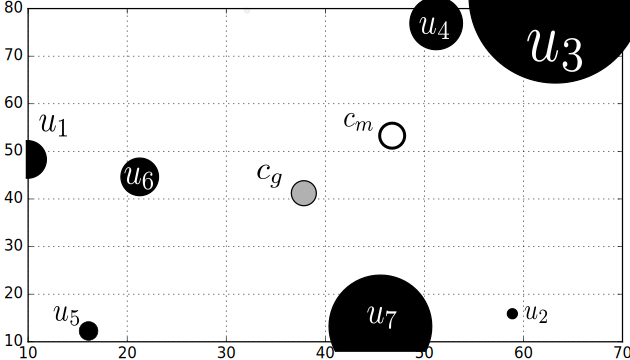
\includegraphics[width=7cm]{img/masses.pdf}
	\caption{$c_m$ is center of mass, $c_g$ is geometric center of black points. 
	Black points radius is its mass. Note the bias given by the weighted sum.}
	\label{fig:masses}       % Give a unique label
\end{figure}

\begin{note}
The bias is given by (\ref{eqn:center}) because for particle with most mass, the 
position of center is nearest to this elements, see Figure \ref{fig:masses}.
\end{note}

\begin{figure}[!ht]
	\sidecaption
	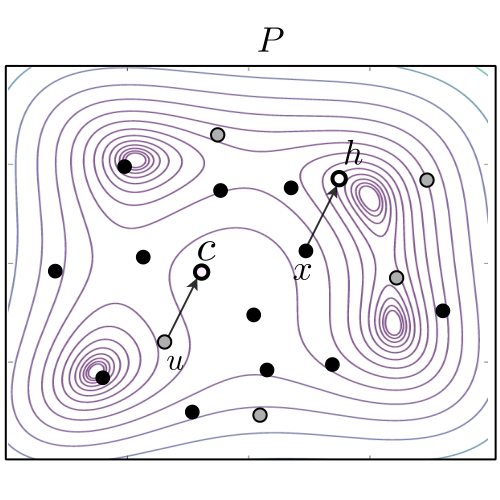
\includegraphics[width=7cm]{img/ecaG.pdf}
	\caption{Schematic diagram representing a generation of ECA. Gray points 
	represent elements in $U$.}
	\label{fig:ecag}       % Give a unique label
\end{figure}

\begin{algorithm}[!ht]
	\caption{Evolution Based on Center of Mass}
	\label{algoritmoEca}
	\begin{algorithmic}[1]
		\Procedure{ECA}{$K = 7, \; \eta_{\max} = 2$}
		%\State poplulation size = 20 $\times$ dimension
		\State $N \gets 2K * D$
		\State Generate and evaluate start population $P$ with $N$ elements
		\While{the end criterion is not achieved}
			\State $A = \emptyset$
			\For {each $\vec{x}$ in $P$}
				\State Generate $U \subset P$ such that  card$(U) = K$
				\State Calculate $\vec{c}$ a using $U$ with (\ref{eqn:center})
				\State $\eta \gets \text{rand}(0,\; \eta_{\max}) $ 
				\State $\vec{h} \gets \vec{x} + \eta  * (\vec{c} - \vec{u}) $ where $ \vec{u} \in U $ random
				
				\If{$ f(\vec{x}) < f(\vec{h})  $}
					\State Append $\vec{h} $ in $A$
				\EndIf
			\EndFor
			\State $P \gets $ best elements in $P \cup A$
			% \State 
		\EndWhile
		\State Report best solution in $P$
		\EndProcedure
	\end{algorithmic}
\end{algorithm}

Note that the ECA algorithm has only two parameters, where $K$ controls the selection 
of neighbors and $\eta_{\max}$ is the largest step that will give each particle. 
For large values of $K$, ECA could converge prematurely, we suggest $K = 7$ a number 
obtained experimentally. Figure \ref{fig:ecag} shows a representations of ECA particle update. 

\subsection{Experiments} % (fold)
\label{sub:experiments}

The Algorithm \ref{algoritmoEca} details the procedure for the correct implementation 
of ECA. On the other hand, using this structure experiments were performed on a 
set of problems with interesting properties.\\

An implementation of this algorithm was performed in the C programming language 
and it was tested with the set of functions of CEC 2017 benchmark \cite{cec2017}. 
Those problems was treated as black-box problems. The explicit equations of the 
problems were not used. The ECA algorithm was programmed in C language using a PC 
with quad-core 2.4 GHz CPU and 8 GB of RAM.\\


\begin{table}[!ht]
	\centering
	\caption{Some function from CEC17 benchmark. This set of functions are shifted 
	and rotated. The search range is $[-100,\; 100]^D$.}
	\label{tab:funcs}
	\begin{tabular}{llcc}
		\hline
		Function & Formula  & Optimal  \\ \hline
		Bent Cigar Function & $ \displaystyle f_1(\vec{x}) = x_1 + 10^6 \sum_{i=2}^D x_i^2 $  & 100 \\ \hline
		%%%%%%%%%%%%%%%%%%%%%%%%%%%%%%%%%%
		Sum of Different Power Function & $ \displaystyle f_2(\vec{x}) = \sum_{i=1}^D |x_i|^{i+1} $  & 200 \\ \hline
		%%%%%%%%%%%%%%%%%%%%%%%%%%%%%%%%%%
		Zakharov Function & $ \displaystyle f_3(\vec{x}) =  \sum_{i=1}^D x_i^2 + \left(\sum_{i=1}^D 0.5x_i\right)^2 + \left(\sum_{i=1}^D 0.5x_i\right)^4 $  & 300 \\ \hline
		%%%%%%%%%%%%%%%%%%%%%%%%%%%%%%%%%%
		Rastrigin’s Function & $ \displaystyle f_5(\vec{x}) =  10D + \sum_{i=1}^D (x_i^2 - 10\cos(2\pi x_i)) $  & 500 \\ \hline
		%%%%%%%%%%%%%%%%%%%%%%%%%%%%%%%%%%
		High Conditioned Elliptic Function & $ \displaystyle f_{11}(\vec{x}) =  \sum_{i=1}^D (10^6)^{\dfrac{i-1}{D-1}} x_i^2 $  & 1100 \\ \hline
		%%%%%%%%%%%%%%%%%%%%%%%%%%%%%%%%%%
		Discus Function & $ \displaystyle f_{12}(\vec{x}) = 10^6 x_1^2 +\sum_{i=2}^D x_i^2 $  & 1200 \\ \hline
		%%%%%%%%%%%%%%%%%%%%%%%%%%%%%%%%%%
		Griewank’s Function & $ \displaystyle f_{15}(\vec{x}) =  \sum_{i=1}^D \dfrac{x_i^2}{4000} - \prod_{i=1}^D \cos\left( \dfrac{x_i}{\sqrt{i}} \right) + 1 $  & 1500 \\ \hline
		%%%%%%%%%%%%%%%%%%%%%%%%%%%%%%%%%%
	\end{tabular}
\end{table}


For this algorithm, $D = 10$ was considered. Here, the optimal values for each 
function are known (see Table \ref{tab:funcs}). There is also a maximum number of 
evaluations equal to \textit{max\_nfes} $= D \times 10,000$.\\

The parameters in all experiments were: $K = 7$, $\eta_i$ is a uniform random number 
between in (0, 2]. The size of the population in each dimension was $N = 2K * D $.

% subsection algorithm_description (end)


% subsection experiments (end)

% section eca (end)



\section{Results} % (fold)
\label{sec:results}

Results of ECA are in Table \ref{tab:eca}, note that ECA could be an excellent 
solution for optimization problems because using few evaluations we have acceptable 
solutions respect to jSO. We compared ECA with jSO (best solution for CEC17 benchmark) 
for 51 independent runs in Table \ref{tab:jso}, we obtained interesting and numerically 
similar results to jSO, although this version of differential evolution is adaptive.\\

Figure \ref{fig:converg} shows divergence graphs. This shows that ECA converges 
fast and this shows that ECA converges fast and this sometimes is good for having 
quick results in real world application. Compare ECA with jSO shows that this strategy 
could be improved with some  self-adaptation technique and thus obtain better results.

\begin{figure}[!ht]
\includegraphics[width=\linewidth]{img/converg.pdf}
\caption{Convergence graphs at median for 51 independent runs. Showing logarithm 
of the error for visualization purposes.}
\label{fig:converg}       % Give a unique label
\end{figure}
\begin{table}[!ht]
\centering
\caption{Results of 51 independent runs of ECA on CEC17 problems for $D=10$.}
\label{tab:eca}
\scalebox{0.7}{
	\renewcommand{\arraystretch}{1.3}
	\begin{tabular}{p{1cm}p{2.5cm}p{2.5cm}p{2.5cm}p{2.5cm}p{2.5cm}}
		\hline
		\noalign{\smallskip}
		$f$ & Best & Wrost & Median & Mean &  Std. \\
		\noalign{\smallskip}\svhline\noalign{\smallskip}
		$f_{1}$ & 0.00000E$+$00 & 0.00000E$+$00 & 0.00000E$+$00 & 0.00000E$+$00 & 0.00000E$+$00 \\ \hline
		$f_{2}$ & 0.00000E$+$00 & 0.00000E$+$00 & 0.00000E$+$00 & 0.00000E$+$00 & 0.00000E$+$00 \\ \hline
		$f_{3}$ & 0.00000E$+$00 & 0.00000E$+$00 & 0.00000E$+$00 & 0.00000E$+$00 & 0.00000E$+$00 \\ \hline
		$f_{4}$ & 0.00000E$+$00 & 0.00000E$+$00 & 0.00000E$+$00 & 0.00000E$+$00 & 0.00000E$+$00 \\ \hline
		$f_{5}$ & 9.94967E--01 & 1.54772E$+$01 & 7.95967E$+$00 & 7.93134E$+$00 & 3.77745E$+$00 \\ \hline
		$f_{6}$ & 4.74662E--07 & 1.87951E--03 & 1.87537E--05 & 7.68970E--05 & 2.64095E--04 \\ \hline
		$f_{7}$ & 1.11988E$+$01 & 2.87323E$+$01 & 1.82470E$+$01 & 1.79819E$+$01 & 4.13487E$+$00 \\ \hline
		$f_{8}$ & 0.00000E$+$00 & 1.39919E$+$01 & 3.97988E$+$00 & 5.20411E$+$00 & 3.44675E$+$00 \\ \hline
		$f_{9}$ & 0.00000E$+$00 & 0.00000E$+$00 & 0.00000E$+$00 & 0.00000E$+$00 & 0.00000E$+$00 \\ \hline
		$f_{10}$ & 2.48759E$+$01 & 1.08470E$+$03 & 7.38475E$+$02 & 7.15419E$+$02 & 1.72816E$+$02 \\ \hline
		$f_{11}$ & 0.00000E$+$00 & 6.57982E$+$00 & 9.94986E--01 & 1.40699E$+$00 & 1.58245E$+$00 \\ \hline
		$f_{12}$ & 0.00000E$+$00 & 2.55756E$+$02 & 1.14822E$+$02 & 7.23057E$+$01 & 6.74642E$+$01 \\ \hline
		$f_{13}$ & 0.00000E$+$00 & 1.36689E$+$01 & 2.44396E$+$00 & 3.57464E$+$00 & 3.36532E$+$00 \\ \hline
		$f_{14}$ & 0.00000E$+$00 & 9.86504E$+$00 & 9.94959E--01 & 1.62895E$+$00 & 2.14527E$+$00 \\ \hline
		$f_{15}$ & 4.70850E--03 & 3.29460E$+$00 & 1.13397E$+$00 & 1.03424E$+$00 & 7.22193E--01 \\ \hline
		$f_{16}$ & 3.90059E--01 & 2.42227E$+$01 & 2.14109E$+$00 & 3.42342E$+$00 & 3.81635E$+$00 \\ \hline
		$f_{17}$ & 6.04248E$+$00 & 4.77547E$+$01 & 3.68447E$+$01 & 3.65033E$+$01 & 6.29621E$+$00 \\ \hline
		$f_{18}$ & 1.91438E--02 & 2.54001E$+$00 & 4.26493E--01 & 5.91709E--01 & 5.31956E--01 \\ \hline
		$f_{19}$ & 3.15884E--02 & 1.56140E$+$00 & 2.90525E--01 & 5.22549E--01 & 4.57284E--01 \\ \hline
		$f_{20}$ & 1.30976E$+$00 & 4.53821E$+$01 & 2.69242E$+$01 & 2.45399E$+$01 & 9.82172E$+$00 \\ \hline
		$f_{21}$ & 1.00000E$+$02 & 2.04138E$+$02 & 1.00000E$+$02 & 1.02042E$+$02 & 1.44386E$+$01 \\ \hline
		$f_{22}$ & 0.00000E$+$00 & 1.01678E$+$02 & 1.15631E$+$01 & 4.87450E$+$01 & 4.90438E$+$01 \\ \hline
		$f_{23}$ & 3.43302E--08 & 3.20754E$+$02 & 3.09754E$+$02 & 3.03630E$+$02 & 4.32143E$+$01 \\ \hline
		$f_{24}$ & 1.98982E--07 & 3.31138E$+$02 & 1.00000E$+$02 & 1.11616E$+$02 & 5.65212E$+$01 \\ \hline
		$f_{25}$ & 3.97743E$+$02 & 4.43546E$+$02 & 3.98009E$+$02 & 3.99730E$+$02 & 8.83947E$+$00 \\ \hline
		$f_{26}$ & 3.00000E$+$02 & 3.00000E$+$02 & 3.00000E$+$02 & 3.00000E$+$02 & 0.00000E$+$00 \\ \hline
		$f_{27}$ & 3.88861E$+$02 & 3.97791E$+$02 & 3.93436E$+$02 & 3.92839E$+$02 & 1.83721E$+$00 \\ \hline
		$f_{28}$ & 3.00000E$+$02 & 3.00000E$+$02 & 3.00000E$+$02 & 3.00000E$+$02 & 0.00000E$+$00 \\ \hline
		$f_{29}$ & 2.31919E$+$02 & 2.87909E$+$02 & 2.57749E$+$02 & 2.57882E$+$02 & 9.95923E$+$00 \\ \hline
		$f_{30}$ & 3.94649E$+$02 & 4.08051E$+$02 & 3.95237E$+$02 & 3.98513E$+$02 & 5.55498E$+$00 \\ \hline
	\end{tabular}
}
\end{table}

\begin{table}[!ht]
\centering
\caption{Comparison results obtained by ECA and jSO for
$D = 10$. Wilcoxon rank-sum test ($\alpha = 0.05$).}
\label{tab:jso}
\scalebox{0.7}{
	\renewcommand{\arraystretch}{1.3}
	\begin{tabular}{p{1cm}p{2.5cm}p{2.5cm}c}
		\hline
		\noalign{\smallskip}
		$f$ & ECA & jSO  \\
		\noalign{\smallskip}\svhline\noalign{\smallskip}
		$f_{1}$ & 0.00000E$+$00  & 0.00000E$+$00 & $\approx$  \\ \hline
		$f_{2}$ & 0.00000E$+$00  & 0.00000E$+$00 & $\approx$  \\ \hline
		$f_{3}$ & 0.00000E$+$00  & 0.00000E$+$00 & $\approx$  \\ \hline
		$f_{4}$ & 0.00000E$+$00  & 0.00000E$+$00 & $\approx$  \\ \hline
		$f_{5}$ & 7.93134E$+$00  & 1.67777E$+$00 & --  \\ \hline
		$f_{6}$ & 7.68970E--05  & 0.00000E$+$00 & --  \\ \hline
		$f_{7}$ & 1.79819E$+$01  & 1.20817E$+$01 & --  \\ \hline
		$f_{8}$ & 5.20411E$+$00  & 1.91188E$+$00 & --  \\ \hline
		$f_{9}$ & 0.00000E$+$00  & 0.00000E$+$00 & $\approx$  \\ \hline
		$f_{10}$ & 7.15419E$+$02  & 3.83851E$+$01 & --  \\ \hline
		$f_{11}$ & 1.40699E$+$00  & 0.00000E$+$00 & --  \\ \hline
		$f_{12}$ & 7.23057E$+$01  & 3.55067E--01 & --  \\ \hline
		$f_{13}$ & 3.57464E$+$00  & 2.68638E$+$00 & $\approx$  \\ \hline
		$f_{14}$ & 1.62895E$+$00  & 1.36563E--01 & --  \\ \hline
		$f_{15}$ & 1.03424E$+$00  & 3.00324E--01 & --  \\ \hline
		$f_{16}$ & 3.42342E$+$00  & 5.49544E--01 & --  \\ \hline
		$f_{17}$ & 3.65033E$+$01  & 5.25569E--01 & --  \\ \hline
		$f_{18}$ & 5.91709E--01  & 2.17729E--01 & --  \\ \hline
		$f_{19}$ & 5.22549E--01  & 7.72037E--03 & --  \\ \hline
		$f_{20}$ & 2.45399E$+$01  & 3.36657E--01 & --  \\ \hline
		$f_{21}$ & 1.02042E$+$02  & 1.42465E$+$02 & +  \\ \hline
		$f_{22}$ & 4.87450E$+$01  & 1.00000E$+$02 & +  \\ \hline
		$f_{23}$ & 3.03630E$+$02  & 3.01261E$+$02 & --  \\ \hline
		$f_{24}$ & 1.11616E$+$02  & 2.96919E$+$02 & +  \\ \hline
		$f_{25}$ & 3.99730E$+$02  & 4.12195E$+$02 & +  \\ \hline
		$f_{26}$ & 3.00000E$+$02  & 3.00000E$+$02 & $\approx$  \\ \hline
		$f_{27}$ & 3.92839E$+$02  & 3.89468E$+$02 & --  \\ \hline
		$f_{28}$ & 3.00000E$+$02  & 3.40596E$+$02 & +  \\ \hline
		$f_{29}$ & 2.57882E$+$02  & 2.34365E$+$02 & --  \\ \hline
		$f_{30}$ & 3.98513E$+$02  & 3.94521E$+$02 & --  \\ \svhline
			Mean & 116.9022       & 99.03207 & \\ \svhline
	\end{tabular}
}
\end{table}


% section results (end)

\section{Conclusions} % (fold)
\label{sec:conclusions}

A new meta-heuristic optimization algorithm, denoted as Evolutionary Centers 
Algorithm, was proposed inspired by center of mass of a system of particles. 
The results showed the capability of the ECA algorithm to reach the global optima 
with greater performance. Also, ECA algorithm obtained results numerically similar 
to jSO and in some cases ECA was significantly better than this version of differential 
evolution.\\

On the other hand ECA uses two parameters, which means that the parameters 
configuration could be simple for other problems. Also, the implementation is not  
complicated. In conclusion ECA is a powerful and promising optimization method for 
solving complicated engineering optimization problems.

% section conclusions (end)

\section{Further Work} % (fold)
\label{sec:further_work}

Implement a self-adaptation technique for solving CEC17 benchmark and obtain 
competitive results. Apply this algorithm in real world problems and justify 
this methodology. Also, we will extend ECA to constrained optimization problems 
and make an analysis about this.

% section further_work (end)

\clearpage
\bibliographystyle{plain}
\bibliography{references}


\end{document}
